\section{Estado del arte}

\begin{frame}{Morfogénesis}
	\begin{center}
		\begin{figure}[htbp]
			\centering
			
\includegraphics[width=0.6\linewidth]{images/morfogenesis.png}
			\caption{Evolución del \textit{emoji} de una lagartija a partir de una única célula activa después de 219 pasos evolutivos \cite{mordvintsevNCA}.}
		\end{figure}
	\end{center}
\end{frame}

\begin{frame}{MNIST}
	\begin{center}
		\begin{figure}[htbp]
			\centering
			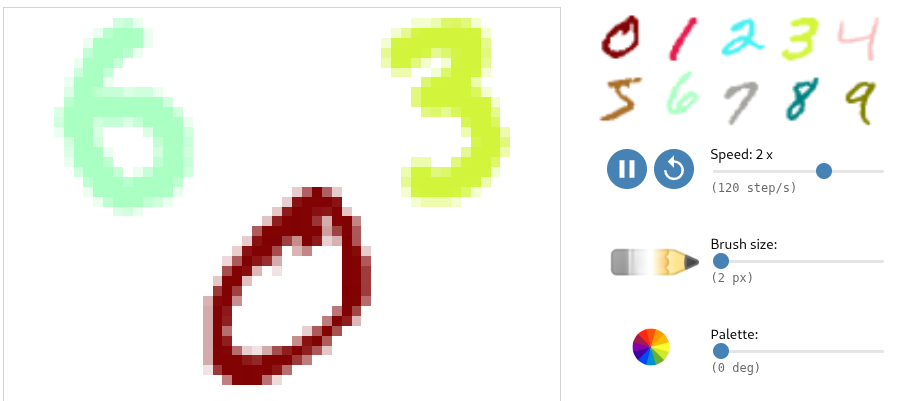
\includegraphics[width=0.6\linewidth]{images/mnist.png}
			\caption{Clasificación de números \cite{MNIST}.}
		\end{figure}
	\end{center}
\end{frame}

\begin{frame}{Mesh}
	\begin{center}
		\begin{figure}[htbp]
			\centering
			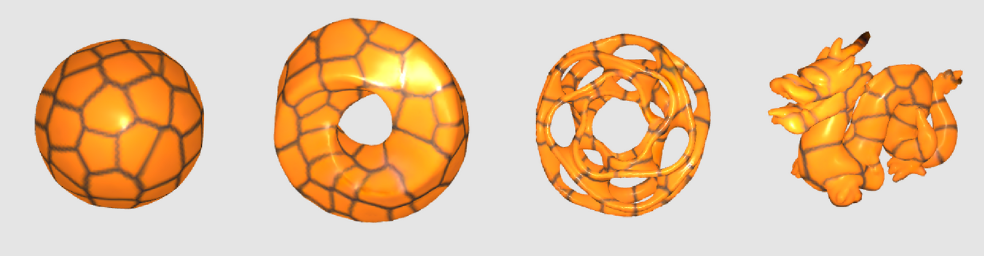
\includegraphics[width=0.6\linewidth]{images/mesh.png}
			\caption{El entrenamiento se realiza sobre un poliedro simétrico y el autómata celular neuronal puede ser extrapolado a cualquier objeto tridimensional \cite{meshNCA}.}
			
		\end{figure}
	\end{center}
\end{frame}
